\documentclass{beamer}
\usepackage{lmodern}% http://ctan.org/pkg/lm
\usepackage{amsmath}
\begin{document}
\title{A Contribution to Rating and Recommendation Systems: Concepts, Development and Evaluation}   
\author{Oliver Diestel} 
\date{\today} 

\frame{\titlepage} 

%\frame{\frametitle{Inhaltsverzeichnis}\tableofcontents} 

\section{Overview} 
\frame{\frametitle{Current Situation (Just an assumption)}
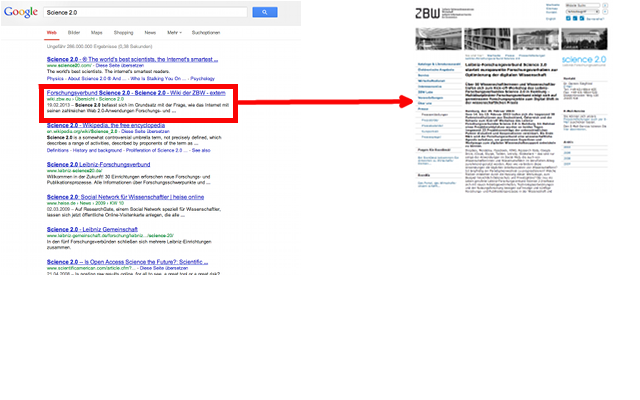
\includegraphics[width=320px, height=200px]{image/google_zbw.png} \\
User visits the zbw.eu website searchs for the information that he would like to have.
Leaves the website.
}
\frame{\frametitle{Possible Situation}
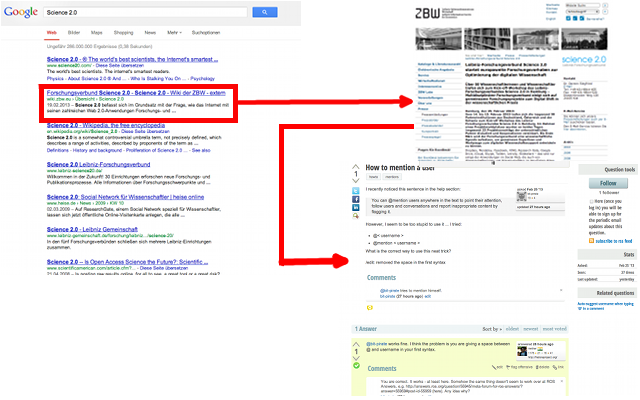
\includegraphics[width=320px, height=200px]{image/google_zbw_askbot.png} \\
User visits the website, sees an interesting question from another user, reads the question and the answer, asks hopefully more questions.
Goal increase the user interaction on a website.
%User visits the zbw.eu website searchs for the information that he would like to have,
%his attention will be drawn to a question from another user that fits the subject and the interest from the user.
%The user visits the site of the question gets a deeper understanding of the subject and asks more questions out of curiosity.


}
\frame{\frametitle{q/A System} 
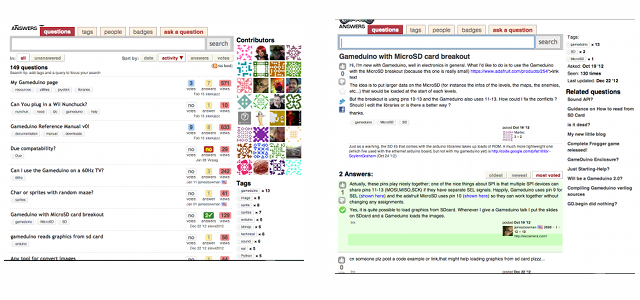
\includegraphics[width=300px]{image/askbot3.png} \\
%Picture of Website / QA with ratings information

%Explanation Question Answer System. (Askbot.com)

General Idea: Use a Question/Answer System(Picture) to make the information retrieval process public.
Use this public questions and answers to increase the user interaction on the website.

%My part is to bring user relevant information that fits the current subject onto a website.
}
\frame{\frametitle{Beginning}
What do we have at the beginning?\\
Website, User and Information(Questions)\\

%After every new concept answer the question what do we have now
}

\section{Rating}
\frame{\frametitle{Rating}
\begin{itemize}
\item Click 
\item active time on page 
\item individual click actions
\end{itemize}

If a user stays shorter or longer on a page than the average user -  
it is a high or low rating.\\
%We rate QA pages and webpages, however we only recommend qa pages.

What do we have now?\\
Questions, Users and the information, which user likes which question 
}

\section{Tagging}
\frame{\frametitle{Tagging}
\begin{itemize}
\item Standard-Thesaurus Wirtschaft, tripple store
\item Stemming: Compute the root of a word. (included in 4-Store)
\item Computing Levenshtein distance: Calculate the distance between two words.
\end{itemize}
\begin{block}{Principle}
Every question will be tagged with a prefered label from the ZBW Thesaurus.\\
For every word in the question find the root of the word and match it against the thesaurus.\\
If we find a matching prefered label, Done. \\
If we find a matching synonym take the preferd label as tag, Done.
\end{block}

What do we have now?
Everything from the beginning + Information about which user likes which question and one or more descriptor that describes the subject of the question

}

\section{Recommendation}

%display this enumeration as a black box
\frame{\frametitle{Input/Output}
Input: $\langle$user\_id, item\_id, rating$\rangle$, [List of tags], number of recommendations\\
Output: Sorted list of Items with avg. rating that correspond with the pref. input label
\begin{itemize}
\item Item: id, name, tag
\item User: id, name
\end{itemize}

Question: How does this black box work?
Three part recommendation. Pipeline architecture
\begin{itemize}
\item Calculate similarity between items
\item Add similar ratings to a user/rating vector.
\item Calculate singular value decomposition
\item Find similar users 
\end{itemize}
}


\frame{\frametitle{Item-Based Algorithm}
Display a matrix with five users and five objects not every user has a rating for every object
To find similar users we need as much user/item ratings as possible so we would like to guess as much ratings as possible.


Find items that have similar ratings.
Calculate the similarity values for every item.
\begin{block}{Cosinus Similarity}
\begin{math}
  sim(\overrightarrow{a}, \overrightarrow{b}) = {\overrightarrow{a} * \overrightarrow{b} \over |\overrightarrow{a}|*|\overrightarrow{b}|}
\end{math}
\end{block}

Take the differences of the average rating behaviour of the user into account.

\begin{block}{Advanced Cosinus Similarity}
\begin{math}
  sim(a, b) = {\sum_{u \in U}(r_{u, a} - \overline{r_u})(r_{u,b} - \overline{r_u}) \over \sqrt{\sum_{u \in U}(r_{u,a} - \overline{r_u})^2} \sqrt{\sum_{u \in U}(r_{u,b} - \overline{r_u})^2 }}
\end{math}
\end{block}

Calculate predictions for similar items.

User u, Product p
\begin{math}
  pred(u, p) = {\sum_{i \in ratedItems(u)} sim(i, p) * r_{u, i} \over \sum_{i \in ratedItems(u)} sim(i, p)}
\end{math}

Fill recommendation vector of each user with similar item ratings 

What do we have now?
Matrix with less empty fields than before.
}

\frame{\frametitle{Singular Value Decomposition}

Now we would like to find similar users with our matrix

Create a SVD with the matrix 
\begin{math}
  M = U * \Sigma * V^t
 \end{math}
 %explanations for u sigma and v
\begin{itemize}
  \item U dimension m x m, orthogonal matrix, spans the column space of matrix m
  \item $\Sigma$ dimension m x n, diagonal matrix having only r nonzero entries
  \item V dimension n x n, orthogonal matrix, spans the row space of matrix m
\end{itemize}
\begin{block}{$\Sigma$ Properties}
  Diagonal entries of $\Sigma$ have the property, that $\sigma > 0$ and $\sigma_i \geq \sigma_{i+1}$
\end{block}
 
 Calculate cosinus similarity between users

 Now we have a two dimensional matrix, so we can calculate the cosinus similarity between our users.
 Display a graph with the users, show which users are similar display the original matrix next to the graph to validate the result.
}

\frame{\frametitle{Is this a good approach?}
  We could have calculated the SVD directly out of the orriginal matrix. Would we get a similar result?
  Is it better if we use the v matrix from the SVD to calculate the item similarity and update the SVD afterwards?
  Is it better if we just recommend similar items from the items the user already likes?
}

\frame{\frametitle{Evaluation}
  The test data: I use real data from the zbw econdesk. However we do not have real user ratings for this data.
  Every data gets a random quality value. 1-5 if a user would rather rate it positive or negative.
  Furthermore I generate 1000 test users these users will have a rating preferation, so a user might be a person that rates an item more positive or more negative.
  I will try to evaluate the algorithms with this test data. I might use a movie db as well for this.

}

\section{Display Information}
\frame{\frametitle{Find Questions}
Find questions that are hightly rated by similar users that match the current topic
}

\frame{\frametitle{Display Questions}
Add a tag and  a div-placeholder on every webpage. Display top questions for the current user on the webpage.

}

\section{Software Architecture}

\frame{\frametitle{Software Architecture}
Scala: Finagle twitter framework\\
Every part of the software is a service.  \\
The tagger, the rating algorithm and the recommendation algorithm can be used as an individual software. \\

Pros:\\
Cons:
}

\section{Timtable}
\frame{\frametitle{Timetable}
Start: 18.12.2012\\
End: 18.06.2012\\

1st month(18.01): Theory\\
2nd month(18.02): Theory + Technology\\ 
3rd month(18.03: Implementation\\
4th month(18.04: Implementation + First writings\\
5th month(18.05): Final thesis\\
Personal Goal\\
Technology implemented: 31.03.2012 \\
Diplom Thesis ready: 01.05.2012
}

% \section{Abschnitt Nr. 2} 
% \subsection{Listen I}
% \frame{\frametitle{Aufz\"ahlung}
% \begin{itemize}
% \item Einf\"uhrungskurs in \LaTeX  
% \item Kurs 2  
% \item Seminararbeiten und Pr\"asentationen mit \LaTeX 
% \item Die Beamerclass 
% \end{itemize} 
% }

% \frame{\frametitle{Aufz\"ahlung mit Pausen}
% \begin{itemize}
% \item  Einf\"uhrungskurs in \LaTeX \pause 
% \item  Kurs 2 \pause 
% \item  Seminararbeiten und Pr\"asentationen mit \LaTeX \pause 
% \item  Die Beamerclass
% \end{itemize} 
% }

% \subsection{Listen II}
% \frame{\frametitle{Numerierte Liste}
% \begin{enumerate}
% \item  Einf\"uhrungskurs in \LaTeX 
% \item  Kurs 2
% \item  Seminararbeiten und Pr\"asentationen mit \LaTeX 
% \item  Die Beamerclass
% \end{enumerate}
% }
% \frame{\frametitle{Numerierte Liste mit Pausen}
% \begin{enumerate}
% \item  Einf\"uhrungskurs in \LaTeX \pause 
% \item  Kurs 2 \pause 
% \item  Seminararbeiten und Pr\"asentationen mit \LaTeX \pause 
% \item  Die Beamerclass
% \end{enumerate}
% }

% \section{Abschnitt Nr.3} 
% \subsection{Tabellen}
% \frame{\frametitle{Tabellen}
% \begin{tabular}{|c|c|c|}
% \hline
% \textbf{Zeitpunkt} & \textbf{Kursleiter} & \textbf{Titel} \\
% \hline
% WS 04/05 & Sascha Frank &  Erste Schritte mit \LaTeX  \\
% \hline
% SS 05 & Sascha Frank & \LaTeX \ Kursreihe \\
% \hline
% \end{tabular}}


% \frame{\frametitle{Tabellen mit Pause}
% \begin{tabular}{c c c}
% A & B & C \\ 
% \pause 
% 1 & 2 & 3 \\  
% \pause 
% A & B & C \\ 
% \end{tabular} }


% \section{Abschnitt Nr. 4}
% \subsection{Bl\"ocke}
% \frame{\frametitle{Bl\"ocke}

% \begin{block}{Blocktitel}
% Blocktext 
% \end{block}

% \begin{exampleblock}{Blocktitel}
% Blocktext 
% \end{exampleblock}


% \begin{alertblock}{Blocktitel}
% Blocktext 
% \end{alertblock}
% }
\end{document}

